\documentclass[a4paper,twosides,openright,titlepage]{book}
\usepackage[italian,english]{babel}
\usepackage[ autostyle,italian=guillemets]{csquotes}
\usepackage[bibstyle=numeric,backend=biber]{biblatex}
\addbibresource{bibliography.bib}

\usepackage{frontespizio}
\usepackage{microtype,amsmath,booktabs,graphicx,fancyhdr}

\newenvironment{abstract}% 
	{\cleardoublepage%
		\thispagestyle{empty}% 
		\null \vfill\begin{center}%
		\bfseries \abstractname \end{center}}% 
	{\vfill\null}


\begin{document}

\begin{frontespizio}
\Istituzione {Politecnico di Milano}
\Divisione{Scuola di Ingegneria Industriale}
\Corso [Laurea Specialistica]{Ingegneria Aeronautica }
\Titoletto {Tesi di laurea:}
\Titolo {Scaling Performance of a DNS \\
 solver written in CPL}
\Candidato{{Mirco Meazzo\\  896195}}
\Relatore {Prof. Maurizio Quadrio}
%\NCorrelatore {Relatore esterno}{Relatori esterni}
\Correlatore{ ...}
\Annoaccademico {2018-2019}
\end{frontespizio} 

\frontmatter
\selectlanguage{english}
\graphicspath{grafici}

\begin{flushright} 
\null\vspace{\stretch{1}}
\pagestyle{empty}
\par Dedicata alla mia famiglia,\par a chi mi ha sempre sostenuto, \par a chi è presente oggi \par e a chi non c'è più
\vspace{\stretch{2}}\null
\end{flushright}




\begin{abstract}
\hrulefill

A numerical method for the direct numerical simulation of the incompressible Navier–Stokes equations in rectangular geometries is presented. The method implement the MPI Standard~\cite{MPI} to the engine developed by M.~Quadrio and P.~Luchini described in~\cite{cpl:presentazione}. 

The method is based on Fourier expansions in the homogeneous directions and fourth-order accurate, compact finite-difference schemes over a variable-spacing mesh in the wall-normal direction. 

Two different versions of the solver have been developed, based on the domain decomposition.  In the first the domain is decomposed through 1D (\emph{Slab}), while in the second version 2D (\emph{Pencil}) decomposition is used.
The performances of these versions have been compared against each other.

To manage the decomposition we rely on the APIs present in \emph{fftMPI}, developed by Steve Plimpton at Sandia National Laboratories~\cite{fftMPI}
\\
\\
\\
\emph{Key words}: Navier–Stokes equations, direct numerical simulation, parallel computing, turbulence, pencil decomposition 

\hrulefill
\end{abstract}




\tableofcontents 
\listoffigures 
\listoftables



\mainmatter
\chapter{Introduction}




\section{Problem Definition}
\pagestyle{headings}

Before moving to what has been done in this thesis I wish to briefly discuss the setup of our channel flow and the equations used to solve the problem.

\begin{figure}[h]
\centering
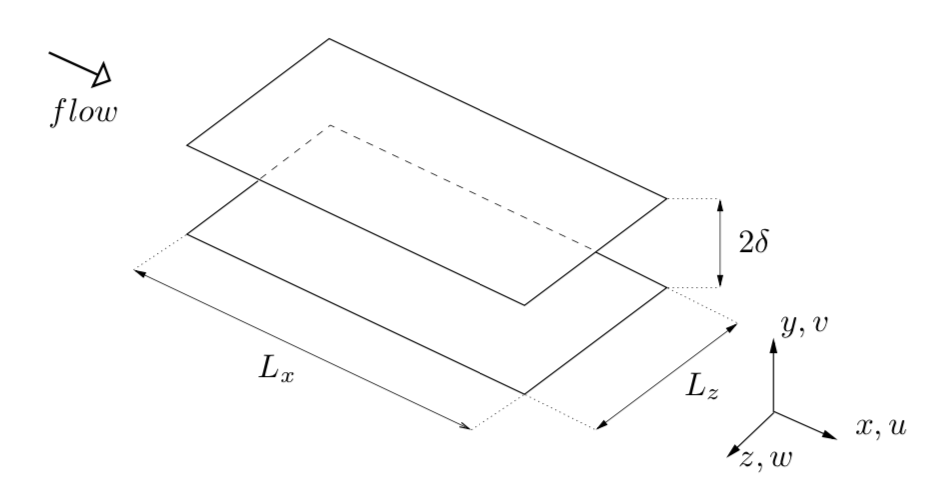
\includegraphics[width=0.8\textwidth]{grafici/sketch_dominio}
\caption{Domain of interest}
\label{sketch_dominio}
\end{figure}

We have the domain sketched in figure~\ref{sketch_dominio} where the $x$ and $z$ coordinates denote the streamwise and spanwise directions of the flow, while the $y$ coordinate is the wall normal ones.
Along these three dimension we have $u,v$ and $w$ components of velocity.

The flow is assumed to be periodic in the streamwise and spanwise directions. The lower wall is at position $y_l$ and the upper wall at position $y_u$. The reference length $\delta$ is taken to be one half of the channel height.
Once an appropriate reference velocity is chosen, we can define the Reynolds number as:
\[
Re = \frac{U\delta}{\nu}
\]
where $\nu$ is the kinematic viscosity of the fluid.

According to our geometry and the assumption of incompressible flow, we can express the behavior of the flow through the mass conservation law:
\begin{equation}
\frac{\partial u}{\partial x} + \frac{\partial v}{\partial y} + \frac{\partial w}{\partial z} = 0
\label{mass:cons}
\end{equation}
 and the Navier-Stokes equations, which in a dimensionless form states:
\begin{subequations}
\label{eqn:ns}
\begin{align}
\frac{\partial u}{\partial t} + u\frac{\partial u}{\partial x} + v\frac{\partial u}{\partial y} + w\frac{\partial u}{\partial z} &= 
- \frac{\partial p}{\partial x} + \frac{1}{Re} \nabla^{2}u  \label{eqn:ns:1}\\
\frac{\partial v}{\partial t} + u\frac{\partial v}{\partial x} + v\frac{\partial v}{\partial y} + w\frac{\partial v}{\partial z} &= 
- \frac{\partial p}{\partial y} + \frac{1}{Re}\nabla^{2}v \label{eqn:ns:2}\\
\frac{\partial w}{\partial t} + u\frac{\partial w}{\partial x} + v\frac{\partial w}{\partial y} + w\frac{\partial w}{\partial z} &= 
- \frac{\partial p}{\partial z} + \frac{1}{Re}\nabla^{2}w \label{eqn:ns:3}
\end{align}
\end{subequations}
The differential problem is closed when an initial condition for all the fluid variables is specified, and suitable boundary conditions are chosen. At the wall the no-slip condition is imposed.








\section{Governing Equations}
The numerical method does not rely on the equations~\eqref{eqn:ns}, instead it solve the wall-normal velocity and the wall-normal vorticity equations, recovering, at the end of the the solution, the three velocity components.\\
\subsection{Wall Normal Vorticity Equation}
Defining the wall-normal component of the vorticity vector as:
\[
\eta = \frac{\partial u}{\partial z} - \frac{\partial w}{\partial x}
\]
which, in Fourier space, holds:
\[
\hat{\eta} = i\beta \hat{u} - i \alpha \hat{w}
\] 
with the hat indicating Fourier-transformed quantities, $i$ the imaginary part, $\alpha$ and $\beta$ the streamwise and spanwise wave numbers;  allows to write a one-dimensional second-order evolutive equation for $\hat{\eta}$ which does not involve pressure, as proposed in \cite{kim_moin_moser}.

Taking the y component of the curl of the momentum equation we obtain:
\begin{equation}
\label{curl:momentum:y}
\frac{\partial \hat{\eta}}{\partial t}  = \frac{1}{Re}  \big( D_{2}(\hat{\eta}) - k^{2} \hat{\eta} \big) + i \beta \widehat{HU} -i \alpha \widehat{HW}
\end{equation}
where $D_{2}$ is the second derivative in the wall-normal direction, $k^{2}$ is the sum of $\alpha$ and $\beta$, and the nonlinear terms are defined as:

\begin{subequations}
\label{nonlinear:terms}
\begin{align}
\widehat{HU} &= i \alpha \widehat{uu} + D_{1} \widehat{uv} + i \beta \widehat{uw}\\ 
\widehat{HV} &= i \alpha \widehat{uv} + D_{1} \widehat{vv} + i \beta \widehat{vw}\\
\widehat{HW} &= i \alpha \widehat{uw} + D_{1} \widehat{vw} + i \beta \widehat{ww}.
\end{align}
\end{subequations}

To solve the equation \eqref{curl:momentum:y} we must set suitable initial conditions for $\hat{\eta}$. Such initial conditions are computed using the initial velocity field and the definition of $\eta$ itself.
Turning such conditions into frequency domain is straightforward and satisfy the periodic boundary conditions. Finally, the \emph{no-slip} condition for velocity vector enforce the condition at the walls, which, simply, translate in $\hat{\eta}=0$ at $y=y_{l}$ and $y=y_{u}$.


\subsection{Wall Normal Velocity Equation}
An equation for the wall-normal velocity component $\hat{v}$, which does not involve pressure, is derived in \cite{kim_moin_moser}, by summing the equation \eqref{eqn:ns:1} derived two times w.r.t. $x$ and $y$, and \eqref{eqn:ns:3} derived two times w.r.t. $y$ and $z$, then subtracting \eqref{eqn:ns:2} derived w.r.t. $x$ and $x$ and substracting once again after derivation w.r.t. $z$ and $z$.
Further simplifications are invoked through the equation \eqref{mass:cons}, which lead to the following fourth-order evolutive equation for $\hat{v}$, which is the so called wall-normal velocity equation:
\begin{equation}
\frac{\partial}{\partial t} \big( D_{2}(\hat{v}) - k^{2} \hat{v} \big) = \frac{1}{Re} \big( D_{4}(\hat{v}) - 2k^{2} D_{2}(\hat{v}) + k^{4} \hat{v} \big)  \\
	-k^{2} \widehat{HV} - D_{1} \big(  i \alpha \widehat{HU} + i \beta \widehat{HW} \big).
\label{normal:velocity}
\end{equation}
To solve such equation we have to enforce initial conditions on $\hat{v}$.\\
According to Fourier expansions, the periodic boundary conditions in the homogeneous directions are automatically satisfied, whereas the no-slip condition for the velocity vector immediately translates in $\hat{v} = 0$ to be imposed at the two walls.\\
The two remaining conditions for the fourth-order equation \eqref{normal:velocity} comes from the continuity equation \eqref{mass:cons}, written at the vertical edges of the domain, $y= y_{l}$ and $y=y_{u}$.


\subsection{Velocity components in the homogeneous directions and Mean flow}
As reported before, once the two preceding equations are solved, we can use them to recover the velocity components in the homogeneous directions.\par
Assuming the non-linear terms \eqref{nonlinear:terms} known, as is the case when such terms are treated explicitly in the time discretization, the equations \eqref{curl:momentum:y} and \eqref{normal:velocity} become uncoupled and, after proper time discretization, can be solved for advancing the solution by one time step, provided the nonlinear terms \eqref{nonlinear:terms} and their spatial derivatives can be calculated.
To this aim, one needs to know how to compute $\hat{u}$ and $\hat{w}$ at a given time starting with the knowledge of $\hat{v}$ and $\hat{\eta}$. \\
By using the definition \eqref{curl:momentum:y} of $\hat{\eta}$ and the continuity equation \eqref{mass:cons} written in Fourier space, a 2 $\times$ 2 algebraic system can be written for the unknowns $\hat{u}$ and $\hat{w}$; its analytical solution read:

\begin{equation}
\begin{cases}
\label{uw:eq}
\hat{u} &= \dfrac{1}{k^{2}} ( i \alpha D_{1}(\hat{v} ) - i \beta \hat{\eta})\\\\
\hat{w} &= \dfrac{1}{k^{2}} (i \alpha \hat{\eta} + i \beta D_{1}(\hat{v}))
\end{cases}
\end{equation}
For $k^{2}=0$ the system of equation \eqref{uw:eq} is singular. \par
The present method therefore enjoys its highest computational efficiency only when Fourier discretization is used in the homogeneous directions.
\par
Since the previous system of equations \eqref{uw:eq} has been obtained starting from equations \eqref{curl:momentum:y} and \eqref{normal:velocity} the solutions are sensible to homogeneous spatial derivatives through the wave numbers. \par
Let us introduce a plane-average operator defined as:
\begin{equation}
\tilde{f} = \frac{1}{L_{x}} \frac{1}{L_{z}} \int_{0}^{L_{x}} \int_{0}^{L_{z}} f \,dx \,dz.
\end{equation}
If we apply such operator to our velocity components vector $\mathbf{V}$, it turns out that $\mathbf{V}(x,y,z,t)~=~\mathbf{\widetilde{V}}(y,t) $. According to this, our velocity components are function of time and wall-normal coordinate only. In Fourier domain this behavior is denoted by the absence of the wave numbers, so for $k^{2}=0$. \par

In agreement with our reference system, where the $x$ axis is aligned with the mean flow, the temporal average of $\tilde{u}$ will denote the mean velocity profile, whereas the temporal average of $\tilde{w}=0$ throughout the channel. \\
Anyway $\tilde{w}$ can be different from zero at different time and distance from the wall. \par

Finally, applying the plane-average operator to the components of the momentum equation let us compute the $\tilde{u}$ and $\tilde{w}$:
\begin{subequations}
\begin{align}
\frac{\partial{ \tilde{u}}}{\partial t} &=  \frac{1}{Re} D_{2} ( \tilde{u}) - D_{1}( \widetilde{uv}) + f_{x} \\
\frac{\partial{ \tilde{w}}}{\partial t} &= \frac{1}{Re} D_{2}( \tilde{w}) - D_{1} ( \widetilde{vw}) + f_{z}
\end{align}
\end{subequations}

 In these expressions, $f_{x}$ and $f_{z}$ are the forcing terms needed to force the flow through the channel against the viscous resistence of the fluid. For the streamwise direction, $f_{x}$ can be an imposed mean pressure gradient, and in the simulation the flow rate through the channel will oscillate in time around its mean value. $f_{x}$ can also be a time-dependent spatially uniform pressure gradient, that has to be chosen in such a way that the flow rate remains constant in time at an imposed. The same distinction applies to the spanwise forcing term $f_{z}$: in this case however the imposed mean pressure gradient or the imposed mean flow rate is zero, while the other quantity will be zero only after time average.


\par
What has been shown in this chapter is intended just to be a brief discussion. Further informations are available in \cite[1-7]{ns:quadrio} and \cite{cpl:presentazione}.







\section{Numerical Method}
the engine of Quadrio and Luchini described into~\cite{cpl:presentazione} which works per \emph{y-slabs}, as shown in figure~\ref{domain_decomp},
\begin{figure}
\centering
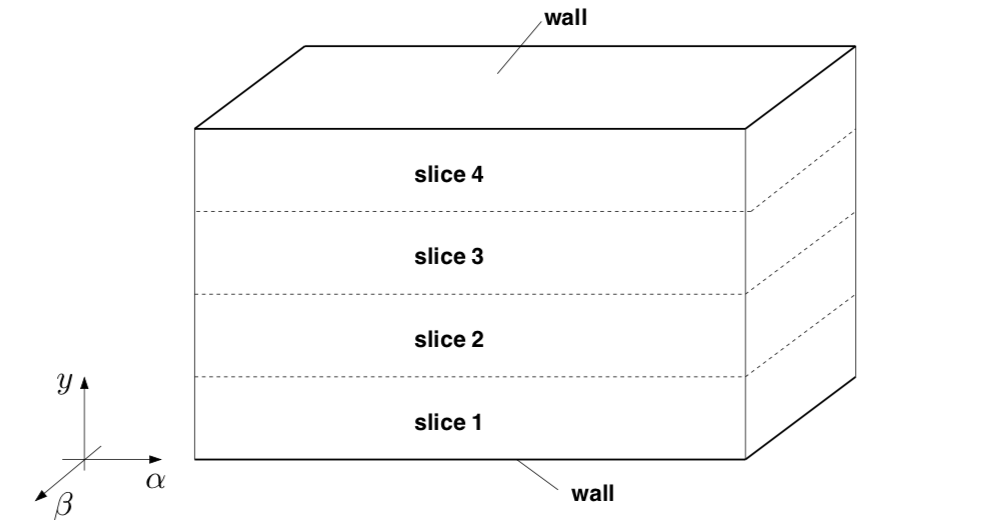
\includegraphics[width=0.5\textwidth]{grafici/decomp_dominio_cpl}
\caption{Original domain decomposition in case of 4 processors}
\label{domain_decomp}
\end{figure} allowing to perform the convolutions and relatives Fourier transformations locally on each processor, leading to a minimum of communication, moving to communication intensive decompositions, such as \emph{z-slabs}, \emph{x-slabs} or \emph{pencils}.

These solutions require communication to perform the array transpose needed by the FFTs in the two homogeneous directions
\chapter{Code Structure}
\section{Spatial discretization along homogeneous directions}
Our solver is based on a Fourier approach. Among the advantages of such approach we face the possibility to expansion of the unknown functions in terms of truncated Fourier series in the homogeneous directions. For example the wall-normal component $v$ of the velocity vector is represented as:
\begin{equation}
v(x,y,z,t) = \sum_{h=-nx/2}^{+nx/2} \sum_{l=-nz/2}^{+nz/2} \hat{v}_{hl}(y,t) e^{i\alpha x}e^{i \beta z}
\end{equation}
where:
\begin{equation}
\alpha = \frac{2\pi h}{L_{x}} = \alpha_{0} h; \quad \beta= \frac{2 \pi l}{L_{z}} = \beta_{0}l
\end{equation}

$h$ and $l$ are integer indexes corresponding to the streamwise and spanwise direction respectively, and $\alpha_{0}$ and $\beta_{0}$ are the fundamental wavenumbers in these directions, defined in terms of the streamwise and spanwise lengths $L_{x} = {2\pi}/{\alpha_{0}} $ and $L_{z} = {2 \pi}/{\beta_{0}}$ of the computational domain. The computational parameters given by the streamwise and spanwise lenght of the computational domain, $L_{x}$ and $L_{z}$ , and the truncation of the series, $nx$ and $nz$, must be chosen so as to miminize computational errors. For further details regarding the proper choice of a value of $L_{x}$ see~\cite{QuadrioMaurizio2003Issi}.

The convolutions required to solve the equations~\ref{curl:momentum:y} and~\ref{normal:velocity} are computationally expensive if carried out in the frequency domain. The same evaluation can be performed efficiently by first transforming the three Fourier components of velocity back in physical space, multiplying them in all six possible pair combinations and eventually retransforming the results into the Fourier space. Fast Fourier Transform algorithms are used to move from Fourier to physical space and viceversa. The aliasing error is removed by expanding the number of modes by a factor of at least $3/2$ before the inverse Fourier transforms, to avoid the introduction of spurious energy from the high-frequency into the low-frequency modes during the calculation~\cite{ns:quadrio}.





\section{Finite difference scheme}
The discretization of the wall-normal derivatives $D_{1}$, $D_{2}$ and $D_{4}$, required for the numerical solution of the present problem, is performed through finite difference (FD) compact schemes~\cite{finite:difference:scheme} with fourth-order accuracy over a computational molecule composed by five arbitrarily spaced grid points. We indicate here with $d_{1}^{j} (i), i = -2, \dots , 2$ the five coefficients discretizing the exact operator $D_{1}$ over five adjacent grid points centered at $y_{j}$ :
\begin{equation}
D_{1} \big( f(y) \big) \vert_{y=y_{j}} = \sum_{i=-2}^{2} d_{1}^{j} (i) f(y_{j+i})
\end{equation}
The basic idea of compact schemes can be most easily understood by thinking of a standard FD formula in Fourier space as a polynomial interpolation of a trascendent function, with the degree of the polynomial corresponding to the formal order of accuracy of the FD formula. Compact schemes improve the interpolation by replacing the polynomial with a ratio of two polynomials, i.e. with a rational function. This obviously increases the number of available coefficients, and moreover gives control over the behavior at infinity (in frequency space) of the interpolant, whereas a polynomial necessarily diverges. This allows a compact FD formula to approximate a differential operator in a wider frequency range, thus achieving resolution properties similar to those of spectral schemes~\cite{finite:difference:scheme}.
Compact schemes are also known as implicit finite-differences schemes, because they typically require the inversion of a linear system for the actual calculation of a derivative~\cite{compact:difference}\cite{finite:difference:scheme}.
 Here we are able to use compact, fourth-order accurate schemes at the cost of explicit schemes, owing to the absence of the third-derivative operator from the equations of motion. Thanks to this property, it is possible to find rational function approximations for the required three FD operators, where the denominator of the function is always the same, as highlighted first in the original Gauss-Jackson-Noumerov compact formulation exploited in his seminal work by Thomas~\cite{Thomas:coeff}, concerning the numerical solution of the Orr-Sommerfeld equations.\par
To illustrate Thomas’ method, let us consider an 4th-order one-dimensional ordinary differential equation, linear for simplicity, in the form:
\begin{equation}
D_{4}(a_{4}f) + D_{2}(a_{2}f)+D_{1}(a_{1}f)+a_{0}f = g,
\label{Thomas:coeff}
\end{equation}
Where the coefficients $a_{i}= a_{i}(y)$ are arbitrary functions of the independent variable $y$, and $g = g(y)$ is a known RHS. Let us moreover suppose that a differential operator, for example $D_{4}$, is approximated in frequency space as the ratio of two polynomials, say $\mathcal{D}_{4}$ and $\mathcal{D}_{0}$. Polynomials like $\mathcal{D}_{4}$ and $\mathcal{D}_{0}$ have their counterpart in physical space, and ${d}_{4}$ and $d_{0}$ are the corresponding FD operators. The key point is to impose that all the differential operators appearing in the example equation~\ref{Thomas:coeff} admit a representation such as the preceding one, in which the polynomial $\mathcal{D}_{0}$ at the denominator remains the same.\par
Equation~\ref{Thomas:coeff} can thus be recast in the new, discretized form:
\begin{equation}
d_{4} (a_{4}f) + d_{2} (a_{3}f) + d_{1} (a_{1}f) + d_{0} (a_{0}f) = d_{0} g,
\end{equation}
and this allows us to use explicit FD formulas, provided the operator $d_{0}$ is applied to the right-hand-side of our equations. The overhead related to the use of implicit finite difference schemes disappears, while the advantage of using high-accuracy compact schemes is retained~\cite{ns:quadrio}.





\subsection{Compute of the finite difference coefficients}










\section{Time Discretization}





\section{Domain Decompositions}
The engine of Quadrio and Luchini described into~\cite{cpl:presentazione} works per \emph{y-slabs}, as shown in figure~\ref{domain_decomp},
\begin{figure}
\centering
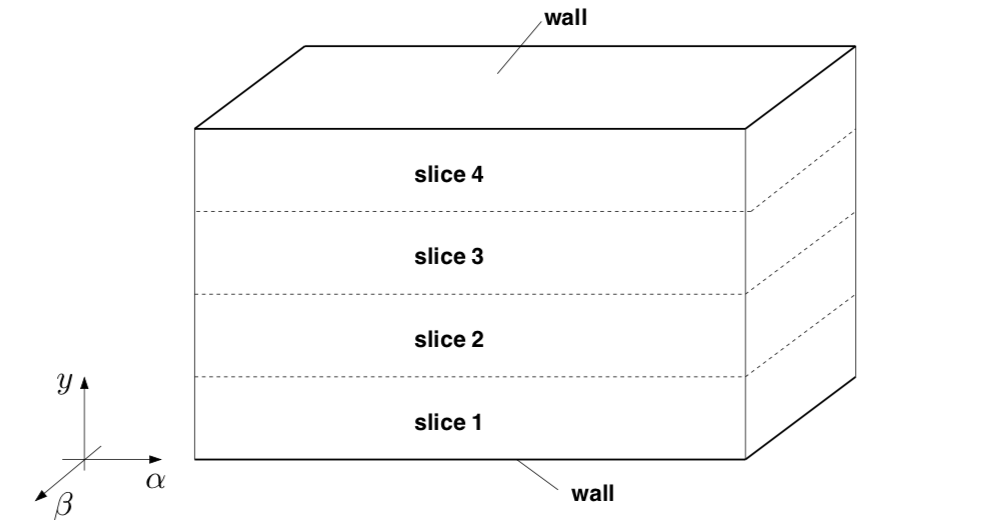
\includegraphics[width=0.8\textwidth]{grafici/decomp_dominio_cpl}
\caption{Original domain decomposition in case of 4 processors}
\label{domain_decomp}
\end{figure}
 allowing to perform convolutions and Fourier transformations locally on each processor, avoiding the cost of non-local transposition for the velocity array and the non-linear terms ones. Such implementation, denominated pipelined-linear-system (PLS), lead to a minimum of communication, in fact this approach require to send and receive only the values stored in the two upper and lower boundary cells of the local decomposition, in order to provide the data required by the fourth-order finite difference scheme.
 \par
 Using the PLS approach the number of bytes exchanged in a three step Range-Kutta method are:
 \begin{equation}
 D_{t} = 3 \times 8 \times (p-1) \frac{3}{2} \times \frac{nx}{p} \frac{nz}{p} \times ny \times 18
 \label{exchange:data:cpl}
 \end{equation}
 where:
 \begin{description}
  \item[3] takes into account the number of time steps;
  \item[8] for counting the bytes;
  \item[$\mathbf{(p-1)}$] is the number of nodes across which the exchange take place;
  \item[ $\mathbf{\frac{3}{2}}$ ] corresponds to the expansion in horizontal modes required by the dealiasing process;
  \item[ $\mathbf{\frac{nx}{p} \times \frac{nz}{p}}$] is the grid portion, for each plane, to exchange with the others nodes;
  \item[18] due to the 3 velocities plus the 6 products to be exchanged twice, before and after the FFT;
  \item[ny] takes into account the number of planes to be exchanged.
\end{description}
Further details about the PLS communications are available in \cite[\nopp chapter 4.2]{ns:quadrio}. \\
 \par
Although efficient for small processors grid, the performances of this approach falls quickly whether the processors number becomes comparable with \emph{ny}.  Furthermore the code structure limit the number of parallel process to be just a fraction of the \emph{ny} extension.
\par
To avoid such limitations and increase the number of parallel processes we decided to move from PLS approach to something different.
We have identified two possible solutions:
\begin{description}
  \item employ \textbf{slab} decomposition along x or z axis;
  \item employ \textbf{pencil} decomposition.
\end{description}
Both implementation require extensive use of the MPI paradigm and, possibly, a library to handle such decompositions.
We opted to employ OpenMPI\cite{openmpi} for what concern the MPI paradigm, in particular we entrust to the well established OpenMPI version 3.1, release 3.1.3.
The ideas behind the choice of such library rely on the fact the OpenMPI is released behind BSD license\cite{bsd:license}, it is designed to group different MPI implementation, avoiding fragmentation and forking problem\cite{faq:openmpi} and, although less optimized on proprietary fabric such as Intel Omni-Path fabric\cite{intel:omnipath}\cite{intel:intelmpivsopenmpi}, is wider spread.


 while, for the decomposition, we entrusted in a new library, released by the 


\subsection{Slabs decomposition}


\subsection{Pencil decomposition}


\chapter{Code Benchmarks}
The following chapter will show the performances obtained after the MPI integration in our code.
We have benchmarked three different problem sizes:
\begin{itemize}
\item small dimension problem $128\times 128 \times 128$;
\item medium dimension problem $512\times 512\times 512$;
\item large dimension problem $4096\times 512\times 512$.  
\end{itemize}
All problems have been tested using 1D and 2D decomposition, so that it is possible to have a comparison among this two methods.
\\
We want to highlight that all these problems exploit the Hermitian symmetry, along the streetwise axis.
\section{Testing environment}
Our test were conducted at CINECA\cite{Cineca}, an Italian academic research center, which host the $19^{th}$ most powerful supercomputers of the TOP500~\cite{top500} of November 2018 list.

We worked on Marconi\cite{marconi:specs} supercomputer, in particular on Marconi-A2 partition.
Marconi structure fuse different partition to reach the peak performance of 20 PFlop/s; in particular our partition is characterized by 3600 nodes, connected through Intel OmniPath\cite{intel:intelmpivsopenmpi} high performance network. Each node host a 68-cores Intel Xeon Phi 7250, code name Knight Landings, and about 100GB of ram. \\
The machine runs on CentOS 7.2~\cite{centos}, a Linux distribution, and our benchmark code has been compiled using GNU GCC 7.3~\cite{gcc} with OpenMPI 3.0.0~\cite{openmpi}\cite{MPI:standard3} . \\
\par
We have tested different flags during the compilation phase, trying to enable different levels of optimization and code vectorization, the most important feature of the Xeon Phi, however the best results have been achieved using:
\begin{lstlisting}
-O2 -fpic -march=native -std=c99
\end{lstlisting}
This behavior was expected since our code does not include the OpenMP\cite{openmp} features at present time, so the MIC\cite{mic} (Many Integrated Cores) architecture can not exploit such fundamental feature, possibly resulting in lack of performances and efficiency.



\section{Scaling performance of $128^3$ problem}
We proceed now showing the performances achieved by our code for the small problem.
This is likely the most critical benchmark for our code, since implement a distributed parallel approach to a problem with tiny dimensions could lead to lack of efficiency quickly. 
\par
In this kind of problem the arrays size fits the cache dimension of the Intel Xeon Phi processor; in fact, we achieve greater speedup by using less nodes as possible at cores equality. For this reason in this test we used 64 cores per node. 
\par
The results of figure \ref{641} shows that, although on single core the structure of the slab decomposed algorithm is faster, suddenly the benefits of pencil decomposition overcome the cost due to the poorer array storage.
To understand the latter sentence we should recall the figure of page \pageref{decomposition:example}.
Keeping in mind figure \ref{decomposition:example}, is possibile to understand why the slab decomposition is faster on single core, and typically also for a tiny cores number. Since the slab algorithm work \emph{per plan} we can, wisely, allocate and work just on a small dataset. This affect the communication phase, which will be faster if compared with the ones of the pencil decomposition that, instead, require to allocate all the data at once. 
\par

\begin{figure}
\begin{center}
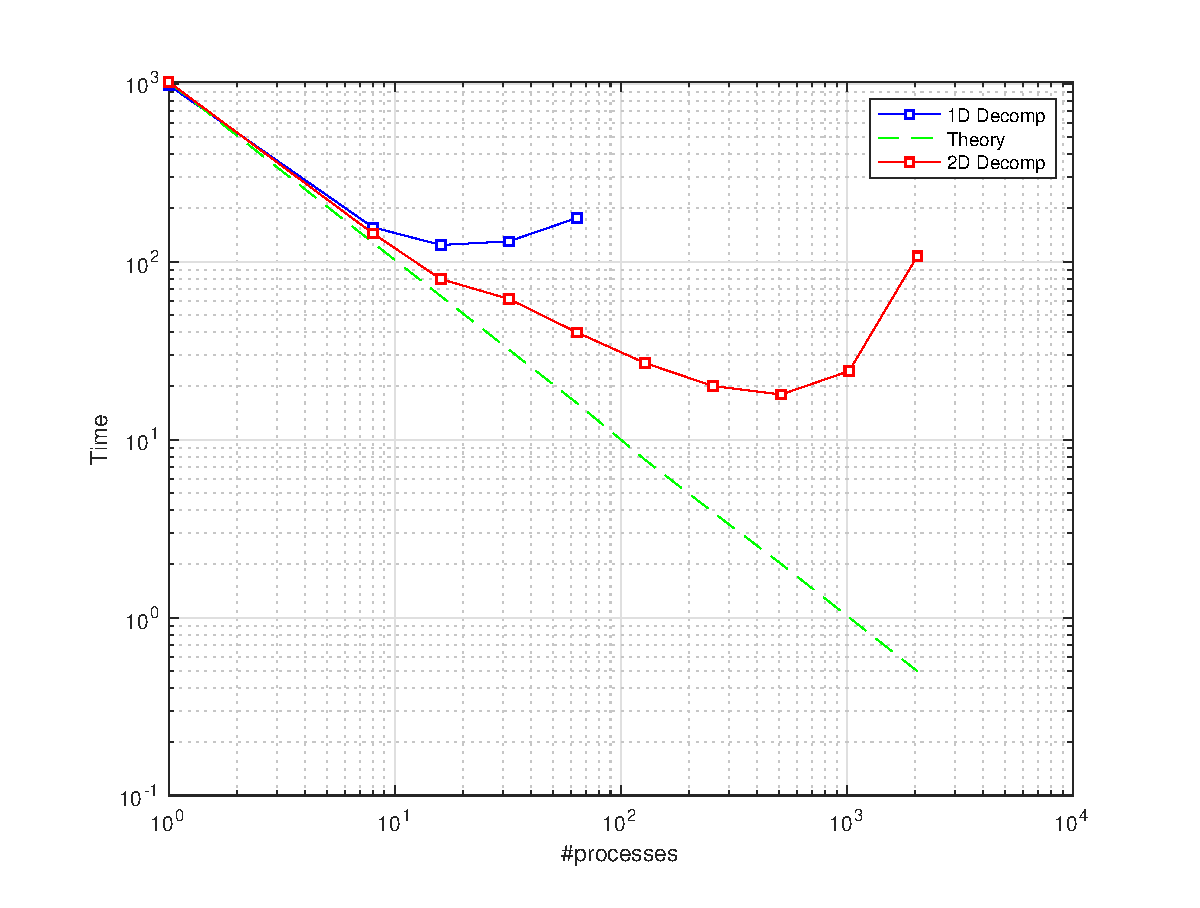
\includegraphics[scale=0.6]{grafici/641}
\caption{Scaling performance of $128^3$ simulation}
\label{641}
\end{center}
\end{figure}

In figure \ref{641} is possible to look at the time needed to perform the DNS, at varying of the cores number and algorithm.
The green dashed line represent the theoretical limit and has been obtained as the ratio between the single core time and the number of cores of the simulation.  \\
Despite of the results could seems poor, the qualitative comparison of figure~\ref{643} against a 3-dimensional FFT, using P3DFFT, reported in \cite[43]{tesi:brach}, suggest that our results are on the average, or better, until the communications cost overcome the benefits of such parallel distributed approach.

\begin{figure}
\begin{center}
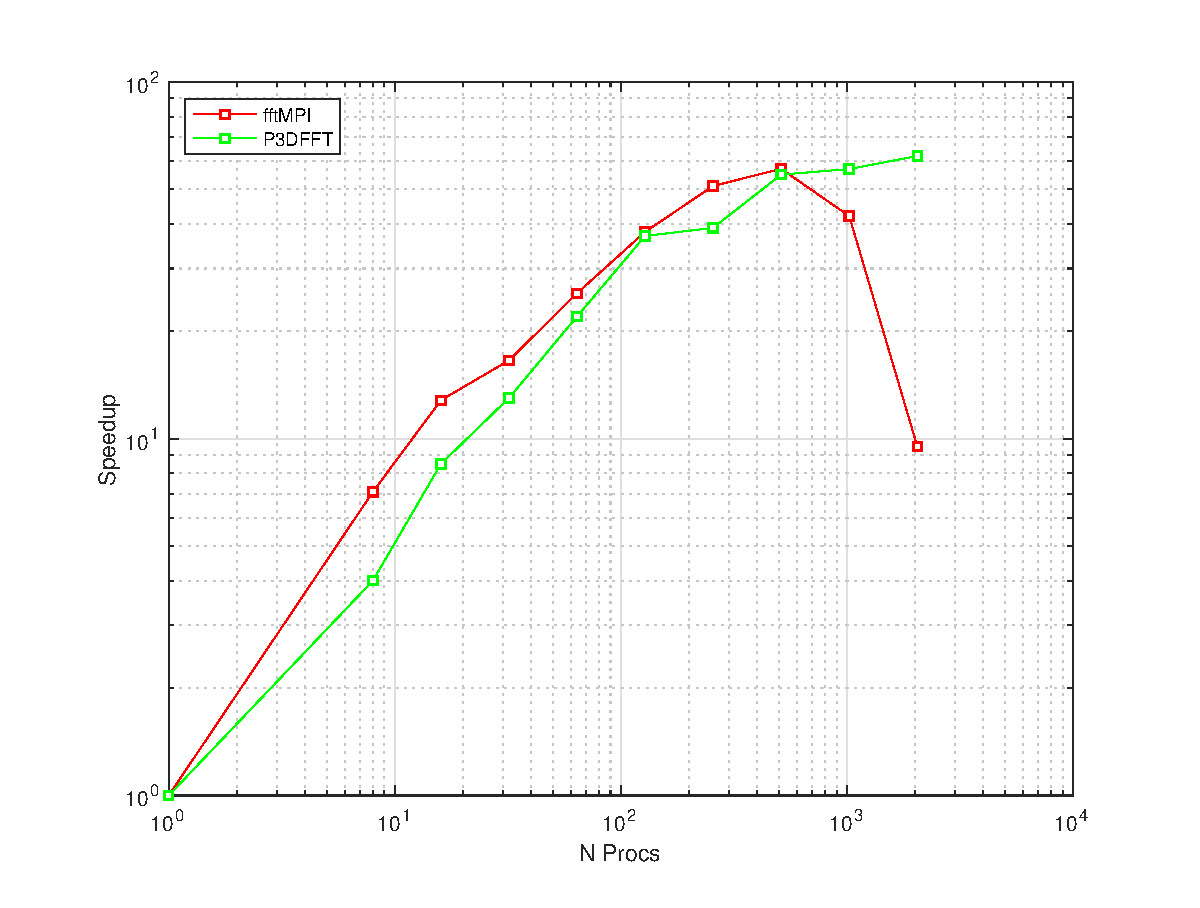
\includegraphics[scale=0.6]{grafici/643}
\caption{Comparison of a 3D FFT against DNS with fftMPI}
\label{643}
\end{center}
\end{figure}

\begin{table}[h]
\caption{Data from $128^{3}$ simulation}
\begin{center}
\begin{tabular}{c c c c}
\toprule
\textbf{\#cores} & \textbf{Time [s]} & \textbf{Speedup} & \textbf{Efficiency [\%]} \\
\midrule
\multirow{2}{*}{1} & 980 & 1.05 & 1.05 \\
& 1022.1 & 1 & 1 \\
\hline
\multirow{2}{*}{8} & 155.9 & 6.56 & 82 \\
& 144 & 7.1 & 89 \\
\hline
\multirow{2}{*}{16} & 124.2 & 8.24 & 52 \\
& 79.73 & 12.82 & 80 \\
\hline
\multirow{2}{*}{32} & 130.4 & 7.86 & 25 \\
& 61.65 & 16.6 & 52 \\
\hline
\multirow{2}{*}{64} & 176.1 & 5.81 & 9 \\
& 39.98 & 25.6 & 40 \\
\hline
128 & 26.9 & 38 & 30 \\

256 & 20 & 51.11 & 20 \\

512 & 17.91 & 57.07 & 11 \\

1024 & 24.28 & 42.1 & 4 \\

2048 & 107.3 & 9.52 & 0 \\
\bottomrule
\end{tabular}
\end{center}
\label{64data}
\end{table}%


The table~\ref{64data} on page~\pageref{64data} summarizes all data related to the $128^{3}$ simulation. 


\par
According to this table the figure \ref{642} shows the speedup at the varying of the cores number. \\
At the speedup peak the code runs $57$ times faster than serial ones. Such peak is obtained using $512$ cores. However, as expectable, the efficiency of this implementation is quite poor. In fact, if we use more than $16$ cores we drop immediately to performances around $50\%$ or lower. 
\par
Such speedup and efficiency have been calculated using the following definitions:
\[
S = \frac{T_{0}}{T_{p}} \quad \quad E = \frac{S}{p}
\]
where $T_{0}$ indicates the single core time, $p$ is the number of cores used in the actual run, and $T_{p}$ is the time associated with it. \\
\par
For completeness the efficiency behavior is reported in figure \ref{644}.

\begin{figure}
\begin{center}
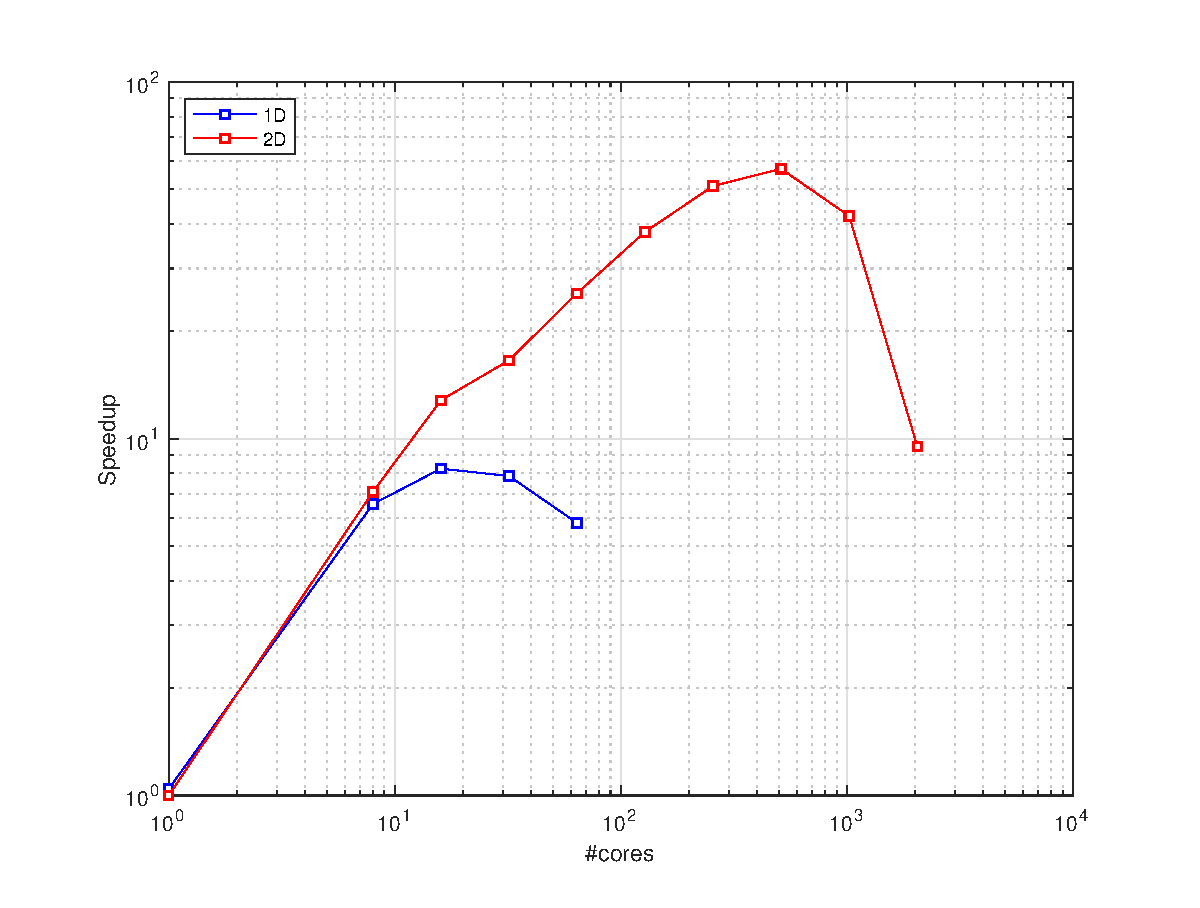
\includegraphics[scale=0.6]{grafici/642}
\caption{Speedup performance $128^3$ simulation}
\label{642}
\end{center}
\end{figure}

\begin{figure}
\begin{center}
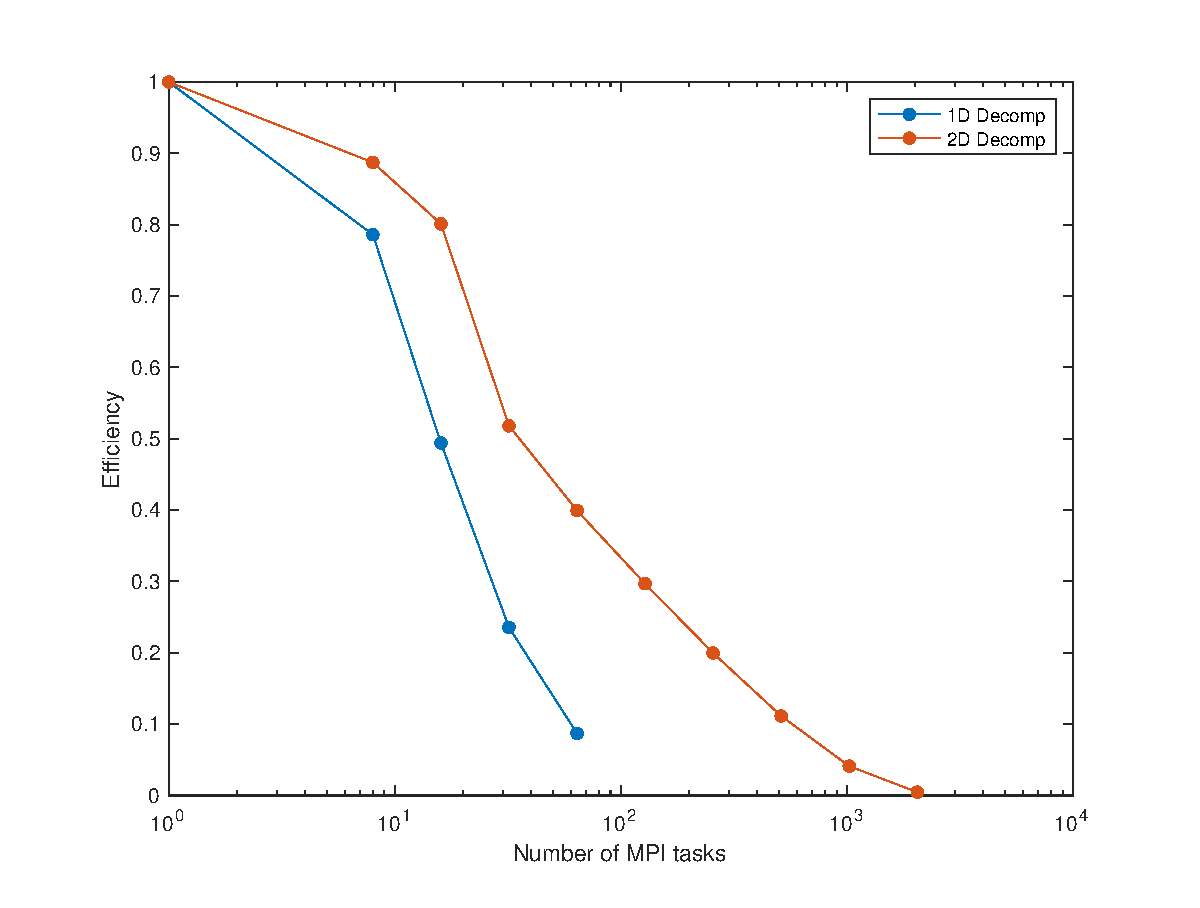
\includegraphics[scale=0.6]{grafici/644}
\caption{Efficiency behavior of $128^3$ simulation}
\label{644}
\end{center}
\end{figure}

\section{Scaling Performance of $512^3$ problem}
\pagestyle{headings}
\section{Scaling Performance of $4096\times512\times256$ problem}
The last benchmark deal with very large problems. Like for the previous large problem, the dimensions are so huge to require the adoption of multiple processors to run, otherwise we will face an out of memory error.
On a Intel Xeon Phi~\cite{intel:xeonphi} the minimum requirements are to employ at least 2 processors and use 32 cores, or less, per processor.
\par
As the previous problem have highlighted, the less cores are used and the better results are scored, so our impossibility to go further than 32 cores per processor, as pointed some rows before, would not be a big deal. We may suppose that the poorest results will be achieved by 32 cores runs, instead of the 64 ones. \\
\par

\begin{figure}
\begin{center}
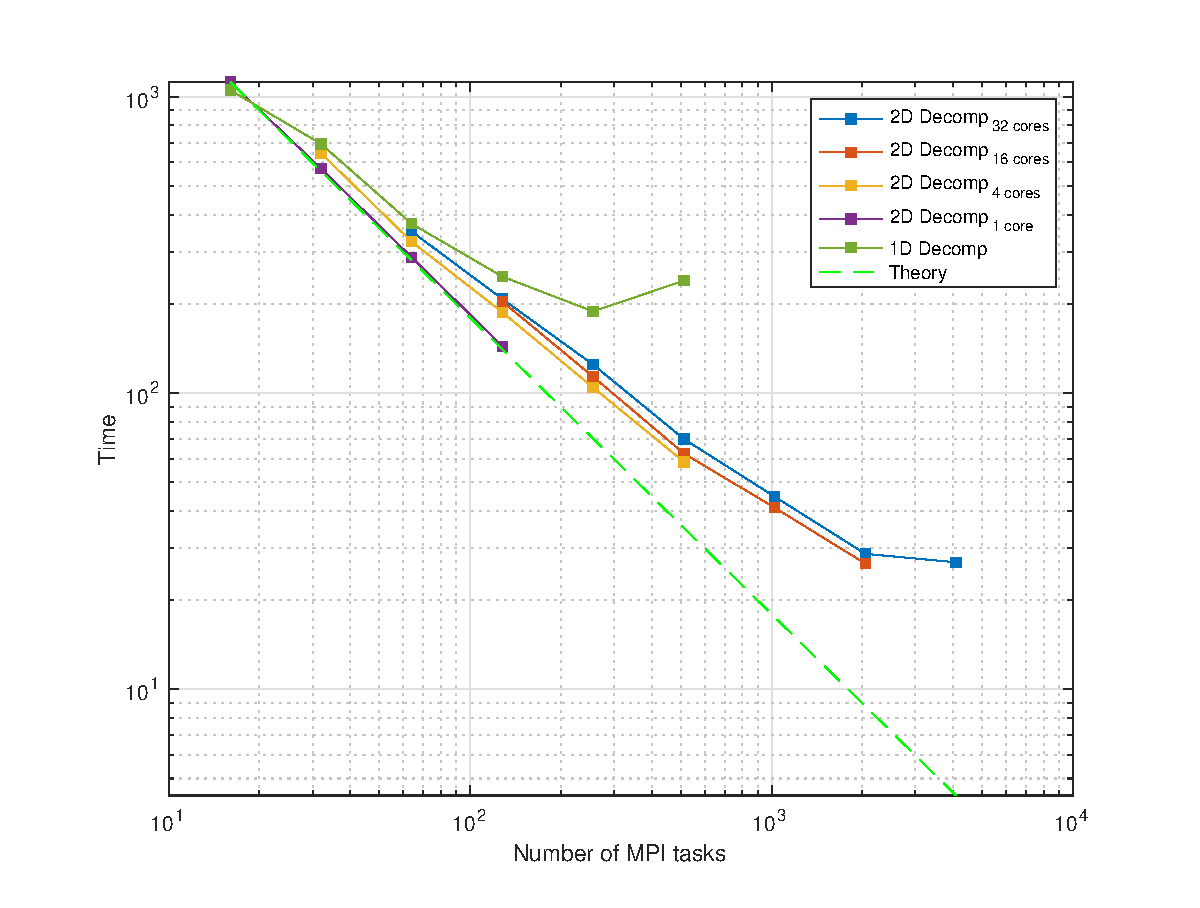
\includegraphics[scale=0.6]{grafici/20481}
\caption{Time scaling comparison for $4096\times 512\times 256$ simulation}
\label{20481}
\end{center} 
\end{figure}

Let us start showing figure~\ref{20481} in which is reported the time scaling of our code.\par
As could be seen, the 2D decomposition using single core achieved the lowest timing execution.
It is interesting to denote how this combination fits the theoretical behavior perfectly.\par
All other 2D decomposed combinations exploit a worse behavior with respect to the single core run, with a marked trend, where the increase in cores per processor number leads to poorer performances. \par 
Such behavior is aligned with our predictions.\\

\begin{figure}
\begin{center}
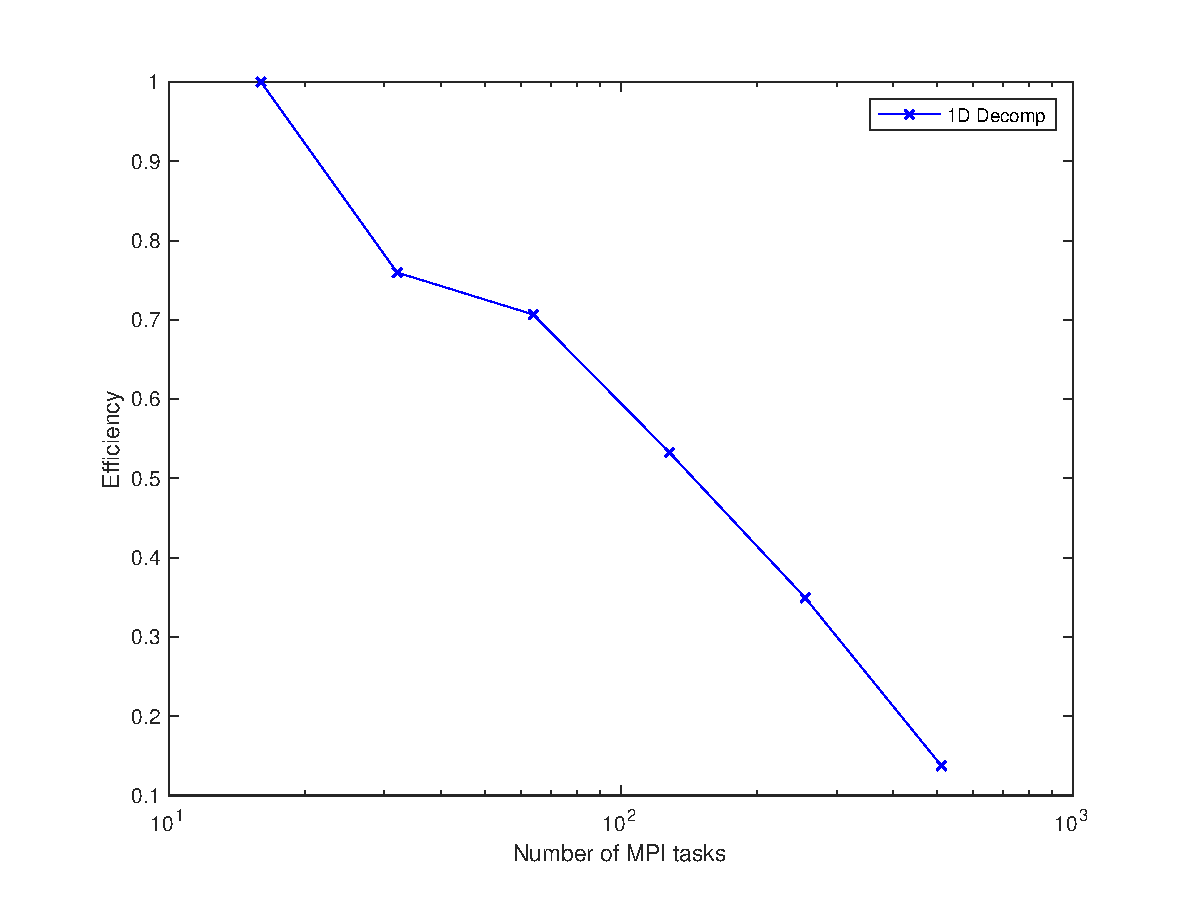
\includegraphics[scale=0.6]{grafici/20483}
\caption{Efficiency factor of $4096\times512 \times256$ simulation using 1D decomposition}
\label{20483}
\end{center}
\end{figure}

\begin{table}
\caption{Data from $4096\times 512\times 256$ simulation, 1D decomposition}
\begin{center}
\begin{tabular}{c c c c}
\toprule
\textbf{\#Processes} & \textbf{Time [s]} & \textbf{Speedup} & \textbf{Efficiency [\%]}\\
\midrule
16 & 1052.9 & 16 & 100\\
32 & 693 & 24.31 & 76\\
64 & 372.5 & 45.23 & 71\\
128 & 247 & 68.2 & 53\\
256 & 188.5 & 89.37 & 35\\
512 & 239.5 & 70.34 & 14\\
\bottomrule
\end{tabular}
\end{center}
\label{2048:data:1}
\end{table}

\par
For what concern about the 1D decomposed algorithm, which, since the code structure is slightly different, can run also on 64 cores per processor, it achieve the worst performances among all possible solutions, highlighting once again the benefits of using a pencil decomposed approach. \par
The speedups achieved by this kind of domain decomposition can be seen in table~\ref{2048:data:1}, on page~\pageref{2048:data:1}, while the efficiency graph, which shows a poor behavior, can be seen in figure~\ref{20483}. \\
\par



Far more interesting, are the data in table~\ref{2048:data:2}, which report the speedups, efficiency and timing achieved by the algorithm with 2D decomposition. The data, and the graphical counterpart which can be seen on page~\pageref{20482} in figure~\ref{20482} and~\ref{20484}, report a very high efficiency using single core, while, although smaller, a still high efficiency is preserved by using 4 cores per processor.\\
\par
\begin{figure}
\begin{center}
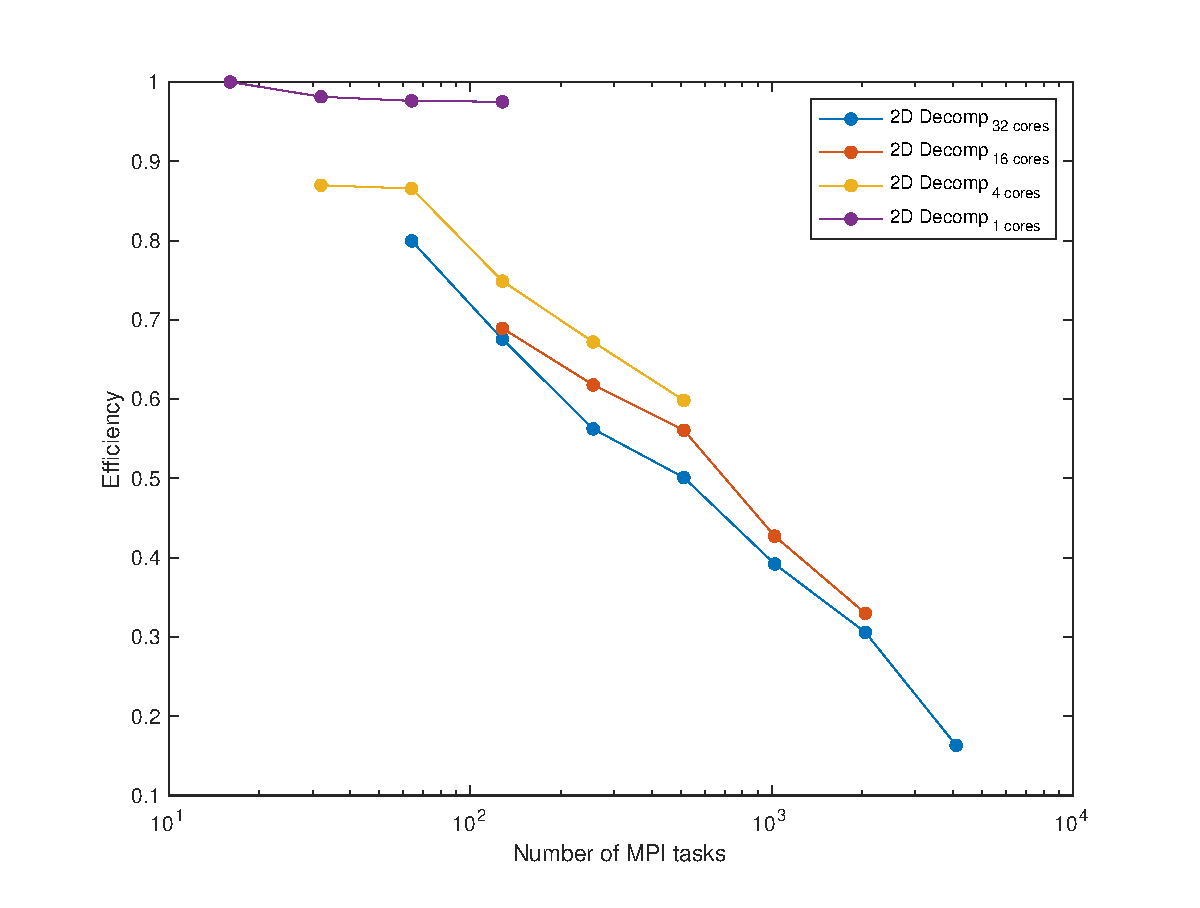
\includegraphics[scale=0.6]{grafici/20484}
\caption{Efficiency factor of $4096\times512 \times256$ simulation using 2D decomposition}
\label{20484}
\end{center}
\end{figure}
Increasing the counter of threads per processor leads to constant losses, as expectable. However, such losses between adjacent stations are lower than the ones of the previous simulations, furthermore we can see wider gaps among the efficiency curves, symptom that there is wider room for improvements.\par
Moreover, at very high number of cores, the efficiency curves slope is minor than before, preserving efficiency and allowing us to perform faster computations with greater speedups.\\
\par
To talk about speedups is useful to introduce figure~\ref{20482}, in which these are reported.\par
The graph, on page~\pageref{20482}, shows the results achieved by the 1D and 2D domain decomposed algorithm, with emphasis on the effects of the variation of cores per processor quantity, for the 2D algorithm only.\par
As has been done in the previous section, the high efficiency shown by the single core run, combined with the physical impossibility to use less cores, has lead us to made the assumption of speedup equal to 16 for a 16 parallel processes run in a single core environment.All other efficiencies and speedups have been derived using such data as reference.\\
\par

\begin{table}
\caption{Data from $4096\times 512\times 256$ simulation, 2D decomposition}
\begin{center}
\begin{tabular}{c c c c c}
\toprule
\textbf{\#Processes} & \textbf{Time [s]} & \textbf{Speedup} & \textbf{Efficiency [\%]} & \textbf{cores}\\
\midrule
16 & 1121.5 & 16 & 100 & 1\\
\hline
\multirow{2}{*}{32} & 571.4 & 31.4 & 98 & 1\\
& 644.8 & 27.83 & 87 & 4\\
\hline
\multirow{3}{*}{64} & 287.2 & 62.47 & 98 & 1\\
& 323.9 & 55.39 & 87 & 4\\
& 350.7 & 51.17 & 80 & 16\\
\multirow{4}{*}{128} & 143.8 & 124.8 & 98 & 1\\
& 187.2 & 95.85 & 75 & 4\\
& 203.4 & 88.23 & 69 & 16\\
& 207.5 & 86.47 & 68 & 32\\
\hline
\multirow{3}{*}{256} & 104.3 & 172 & 67 & 4\\
& 113.4 & 158.2 & 62 & 16\\
& 124.6 & 144 & 56 & 32\\
\hline
\multirow{3}{*}{512} & 58.6 & 306.4 & 60 & 4\\
& 62.5 & 287.1 & 56 & 16\\
& 70 & 256.5 & 50 & 32\\
\hline
\multirow{2}{*}{1024} & 41 & 437.5 & 43 & 16\\
& 44.7 & 401.4 & 39 & 32\\
\multirow{2}{*}{2048} & 26.6 & 675.5 & 33 & 16\\
& 28.7 & 626.3 & 31 & 32\\
\hline
4096 & 26.8 & 668.8 & 16 & 32\\
\bottomrule
\end{tabular}
\end{center}
\label{2048:data:2}
\end{table}

As can be seen in table~\ref{2048:data:2} the best result is achieved using 16 cores per processor and 2048 parallel processes. Unfortunately, due to some policy limitations, we can not push forward our resources request, although the graph clearly shows margins of improvements for such configuration.\\
\par
Differently from all the previous simulations, the processor grid for the pencil decomposition results balanced when the streamwise stencil has half the modes with respect to the other direction. Such configuration has been suggested by benchmarks.
\par
In conclusion we may say that, although the modes distribution results unbalanced in this simulation, the speedup trend still remain aligned with the ones exhibited in the other simulations.
\begin{figure}
\begin{center}
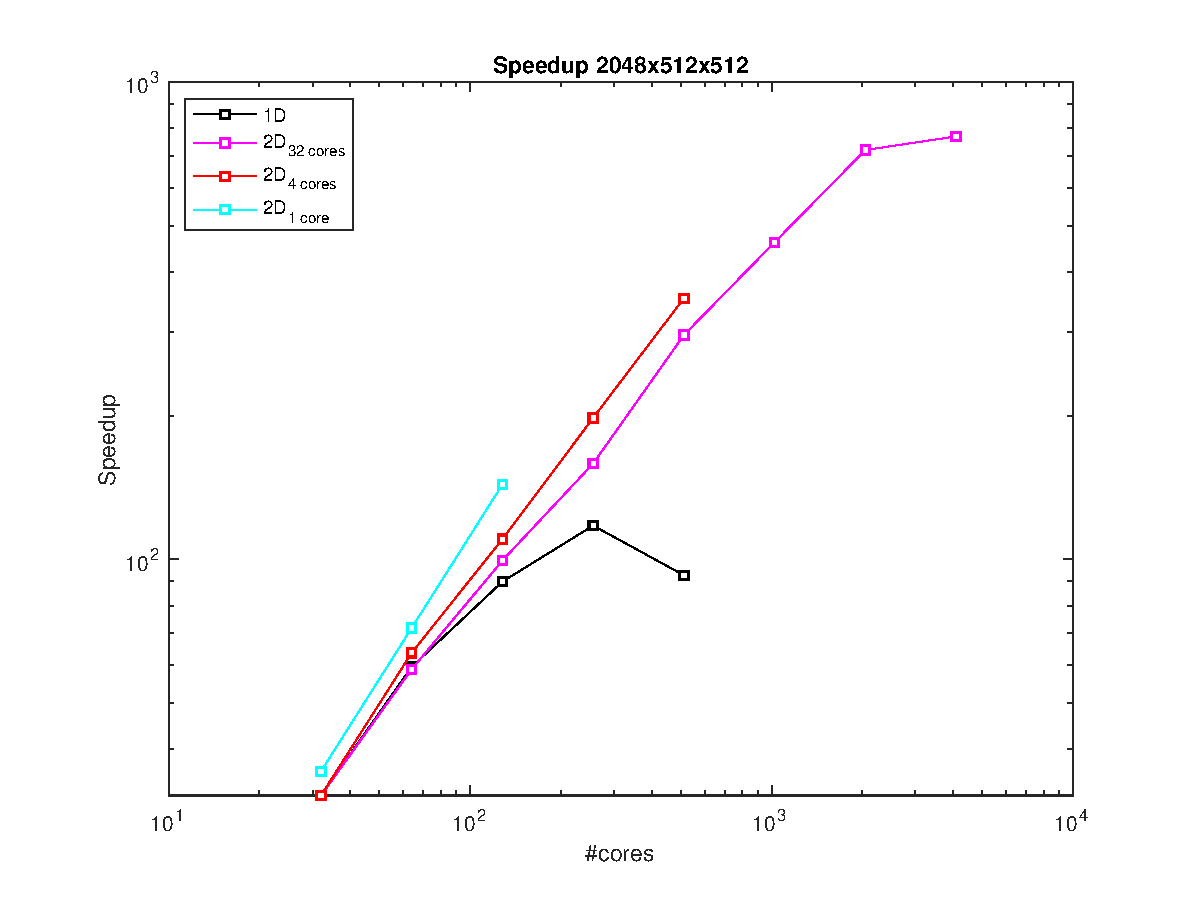
\includegraphics[scale=0.6]{grafici/20482}
\caption{Speedup factor of $4096\times512 \times256$ simulation}
\label{20482}
\end{center}
\end{figure}





\section{Benchmarks conclusions}
The benchmark series has highlighted common trends present in our simulations.
\par
By looking at the curves, we can see that the performances envelope is bordered by the 64 cores run and the single core ones.  We can catch from the graphs that the code tends to perform faster using as less threads per processor as possible.  This behavior is reasonable, since our code and the library in which we rely on to perform the MPI transposition, does not implement the OpenMP technology at the moment, so, although we could carry on the simulation basing our communications on MPI, we will experience efficiency lacks when dealing with intra-node messagings. In particular, when dealing with many cores per processor we face a speedup tendency to pass from 2 to $2^{2/3}$, as the number of MPI tasks gets doubled, as highlighted in~\cite{dns:gpu:supercomputer}. \par
Unfortunately, the Intel KNL's architecture~\cite{intel:xeonphi} is designed to exploit code vectorization as much as possible and OpenMP plays a key role in this kind of implementations. \par
We suggest to move to traditional processors architectures, instead of using MIC, to experience lower losses. Our simulations in fact has highlighted that, although MPI can not guarantee high efficiency in heavily threaded applications, the lacks using 16 cores, or less, per processor can be acceptable.\\
\par
As the problem size grows, the optimal number of MPI tasks, to achieve the best speedup, grows. In fact, we passed from 512 parallel processes for a $128^{3}$ simulation to 2048 for a $512^{3}$ simulation. \par

\begin{figure}
\begin{center}
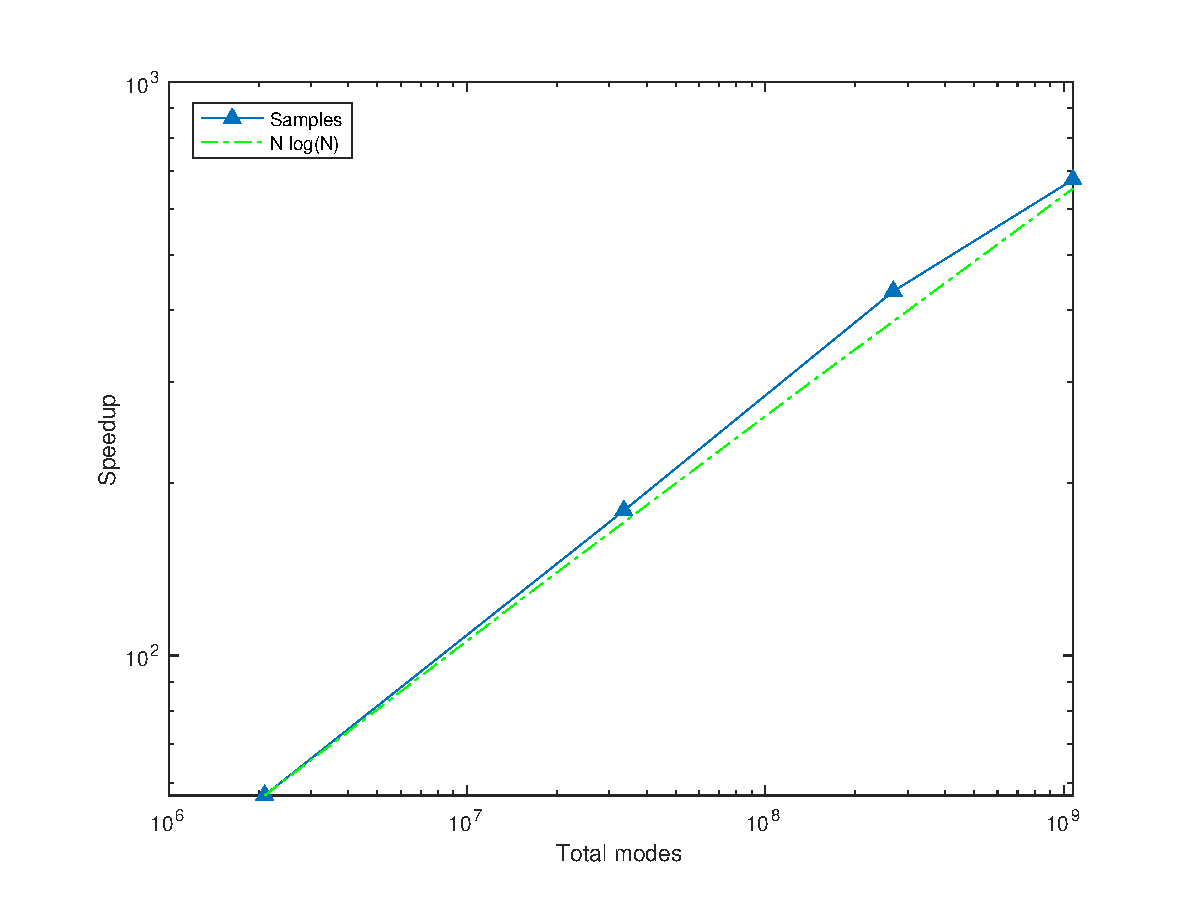
\includegraphics[scale=0.6]{grafici/speedup_trend}
\caption{Speedup factors growth}
\label{speedup:trend}
\end{center}
\end{figure}

On the other hand, the speedup factor increase its peak in a fashion which lies between $N\log(N)$ and $N^{2}$, like testify by figure~\ref{speedup:trend} in which our samples are plotted against such behaviors. \\
\par

\begin{figure}
\begin{center}
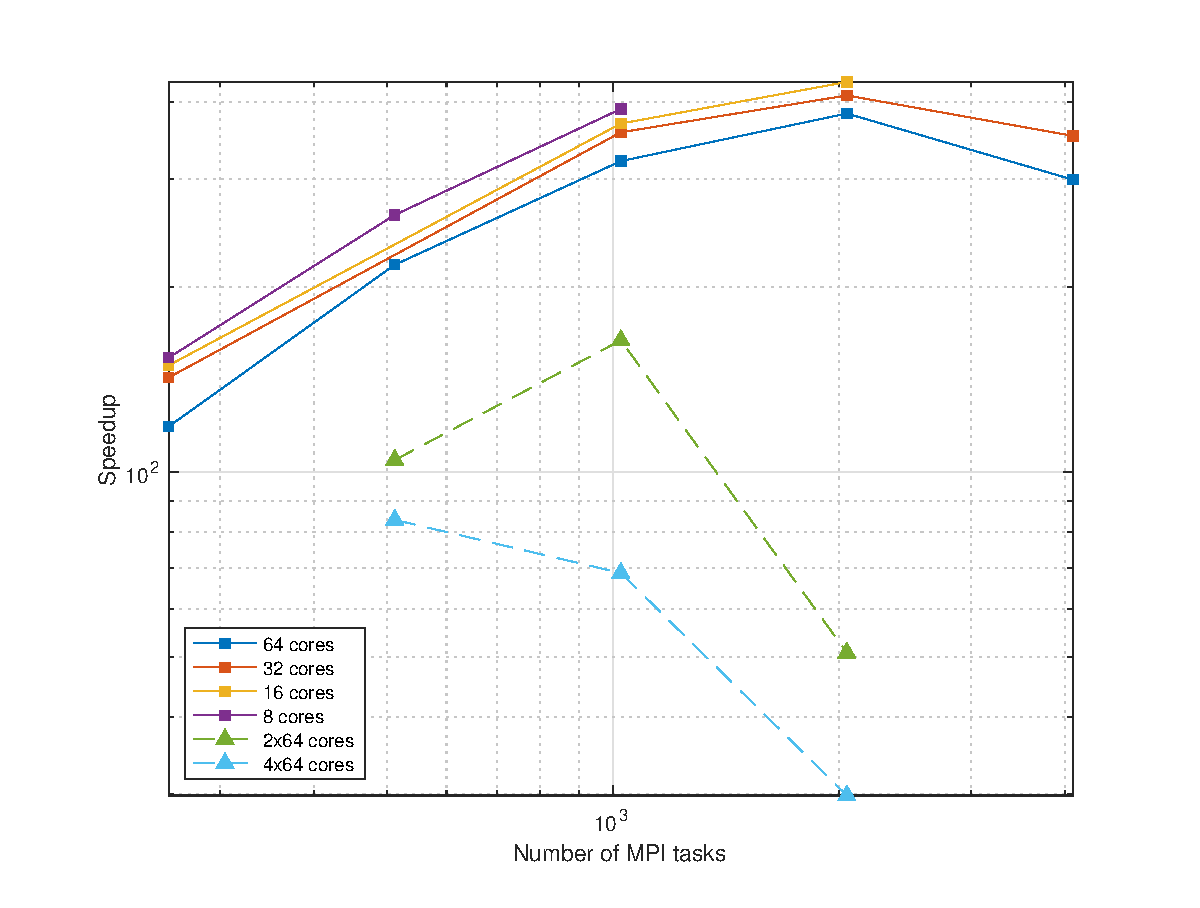
\includegraphics[scale=0.6]{grafici/hyperthreading}
\caption{Hyper threading benchmark}
\label{hyper}
\end{center}
\end{figure}

In conclusion we show the speedup comparison with hyper threading turned on. \par
Hyper threading is a technology~\cite{hyper:paper} developed by Intel that virtually doubles the cores on the CPU, making the CPU run faster and more efficient by scheduling the workload between the cores. On modern Xeon Phi we can quadruplicate the number of cores, obtaining until 272 threads per processor. However, as our benchmark shows, this technology does not provide a boost in terms of speedup, on the contrary it penalizes our results in evident fashion.\par
In figure~\ref{hyper} are compared the original results of a $512^{3}$ simulation, running on different cores per processor, against two curves which exploit the hyper threading technology.


\- Parlare delle dimensioni delle matrice e come ottenere migliori prestazioni \cite{tesi:brach}

\backmatter
\addcontentsline{toc}{chapter}{\bibname} 
\printbibliography

\end{document}
